This section will give an abstract view and an implementation of the proposed data model for the acquired data.
Firstly the current data used in the \project{} will be described after that the data model used for technical implementation will be described.

\section{Data Description}
\label{datamodel-data-description}

There are two types of data in the \project{}, data coming from the \PRN{} and data coming from the clinics.
The \PRN{} data is fairly structured, there are some changes in the data model over time but overall not much is added or removed.
This differs from the clinics which have a great variance in datasets between each other.
During the \project{} a transition is happening, most (if not all) of the clinics will be adopting a new patient record system (LSFD\footnote{http://stichting-saf.nl/lsfd/}).
This system is developed in coordination with the Dutch foundation for automation of fertility clinics (Dutch: Stichting Automatisering Fertiliteit, SAF\footnote{http://stichting-saf.nl/}).
The SAF embodies the interests of all fertility healthcare providers in the Netherlands and therefore they can make decisions on how to standardise datasets.

In the data model of the \ivfsystem{} it should not be required to have one standardised dataset, at the current time (without the LSFD software) there is no standardised dataset.
The knowledge that at one point in time a standard dataset is available should be taken into account but it is more a data gathering problem.

The data itself is provided in a table-like format with columns and rows.
Data was gathered retrospectively and it is retrieved for the year 1999 up to 2010.
Each of the rows contain a pregnancy and each pregnancy consist of data items that are related to it (columns), \eg{} BMI at the time of impregnation.
Between clinics the provided columns differ from each other, during data gathering there was a protocol describing the requested data items but not all clinics were able to provide these.
Data gathered from the \PRN{} registry is available for each of the rows as the requested data items have not changed over the time period (1999 - 2010).
Most of the identifying data has been stripped and those items that remain are pseudonymised, \eg{} the pseudonym for date of birth is age in years.
After this is done the dataset is received by the \ivfsystem{}.

A first step that needs to be performed is to clean the data and make it usable for computerised processing.
The first data clean up will need to be done by hand, but once an algorithm is defined for a specific dataset further updates can be performed automatically.
Datasets that have been cleaned will be stored in the \ivfsystem{} an abstract model will be described in the following section.

\section{Model Description}
\label{datamodel-model-description}

Initially in the \project it is the case that two datasets (\IVF{} and \PRN{} data) will be linked and stored together.
However, the data model has to be flexible in order to make arrangements for future extensions. 
Both in adding new datasets and in extending existing datasets with more data items.

At the start of the project requirements were identified regarding the data storage. 
Requirements were distilled from literature and interviews from the data security section \ref{security}, and also from interviews performed with stakeholders before starting the project.

\begin{enumerate}[topsep=0pt, itemsep=-1ex]
	\item User and role based access to data;
	\item Keep data provenance;
	\item Datasets can be extended with new data items;
	\item New datasets can be added;
	\item Also keep non-linked data in dataset;
	\item Keep linkage between datasets in a separate entity;
	\item Keep data agreements with the datasets;
	\item Aggregated/statistical data retrieval should be possible.
\end{enumerate}

\paragraph{Compiling the model}
\label{datamodel-compiling}

The first data model for the \ivfsystem{} was developed from these requirements and can be seen in figure \ref{fig:model-drawing}.
Complying to requirement 1, 2, 6, and 7 was straightforward, each of the requirements describes that the data should be stored in a separate entities which is reflected in the model.
Data entities are respectively: {\tt User}, {\tt Provenance}, {\tt Linkage}, and {\tt Data agreements}.

Requirement 3 and 4 both have a need for {\tt Sub collections}, these implement a minimum data item set.
For example, one of the {\tt sub collections} is the \IVF{} dataset, the cross section of available data items for all \IVF{} datasets is the minimum data item set.
This set-up makes it possible to add other (different) datasets but also to extend existing datasets with new data items.

Requirement 5 needs some background information.
In the data linkage process not all rows of data from one dataset will find a corresponding row in the other dataset.
Discarding these rows is not in the interest of the research that can be performed on the whole dataset.
This is where requirement 6 comes in to play, keeping the {\tt Linkage} separately from the {\tt Data} makes it possible to keep all rows (including the non-linked).
Incorporating these possibilities into the data model opens up chances for more functionality in the \ivfsystem{}.

Requirement 8 is based on both security as functional considerations.
The security literature tells us that the raw dataset should be protected against direct access as much as possible.
Therefore, when research is performed on the extracted data certain key data items can be aggregated.
This creates a protection layer against identifying individuals in the extracted data.
For example, (most of the time) it is unnecessary to know the exact age for each of the included patients in a research, in those cases the aggregated mean age of all patients can suffice.

\begin{figure}[!b]
	\centering
	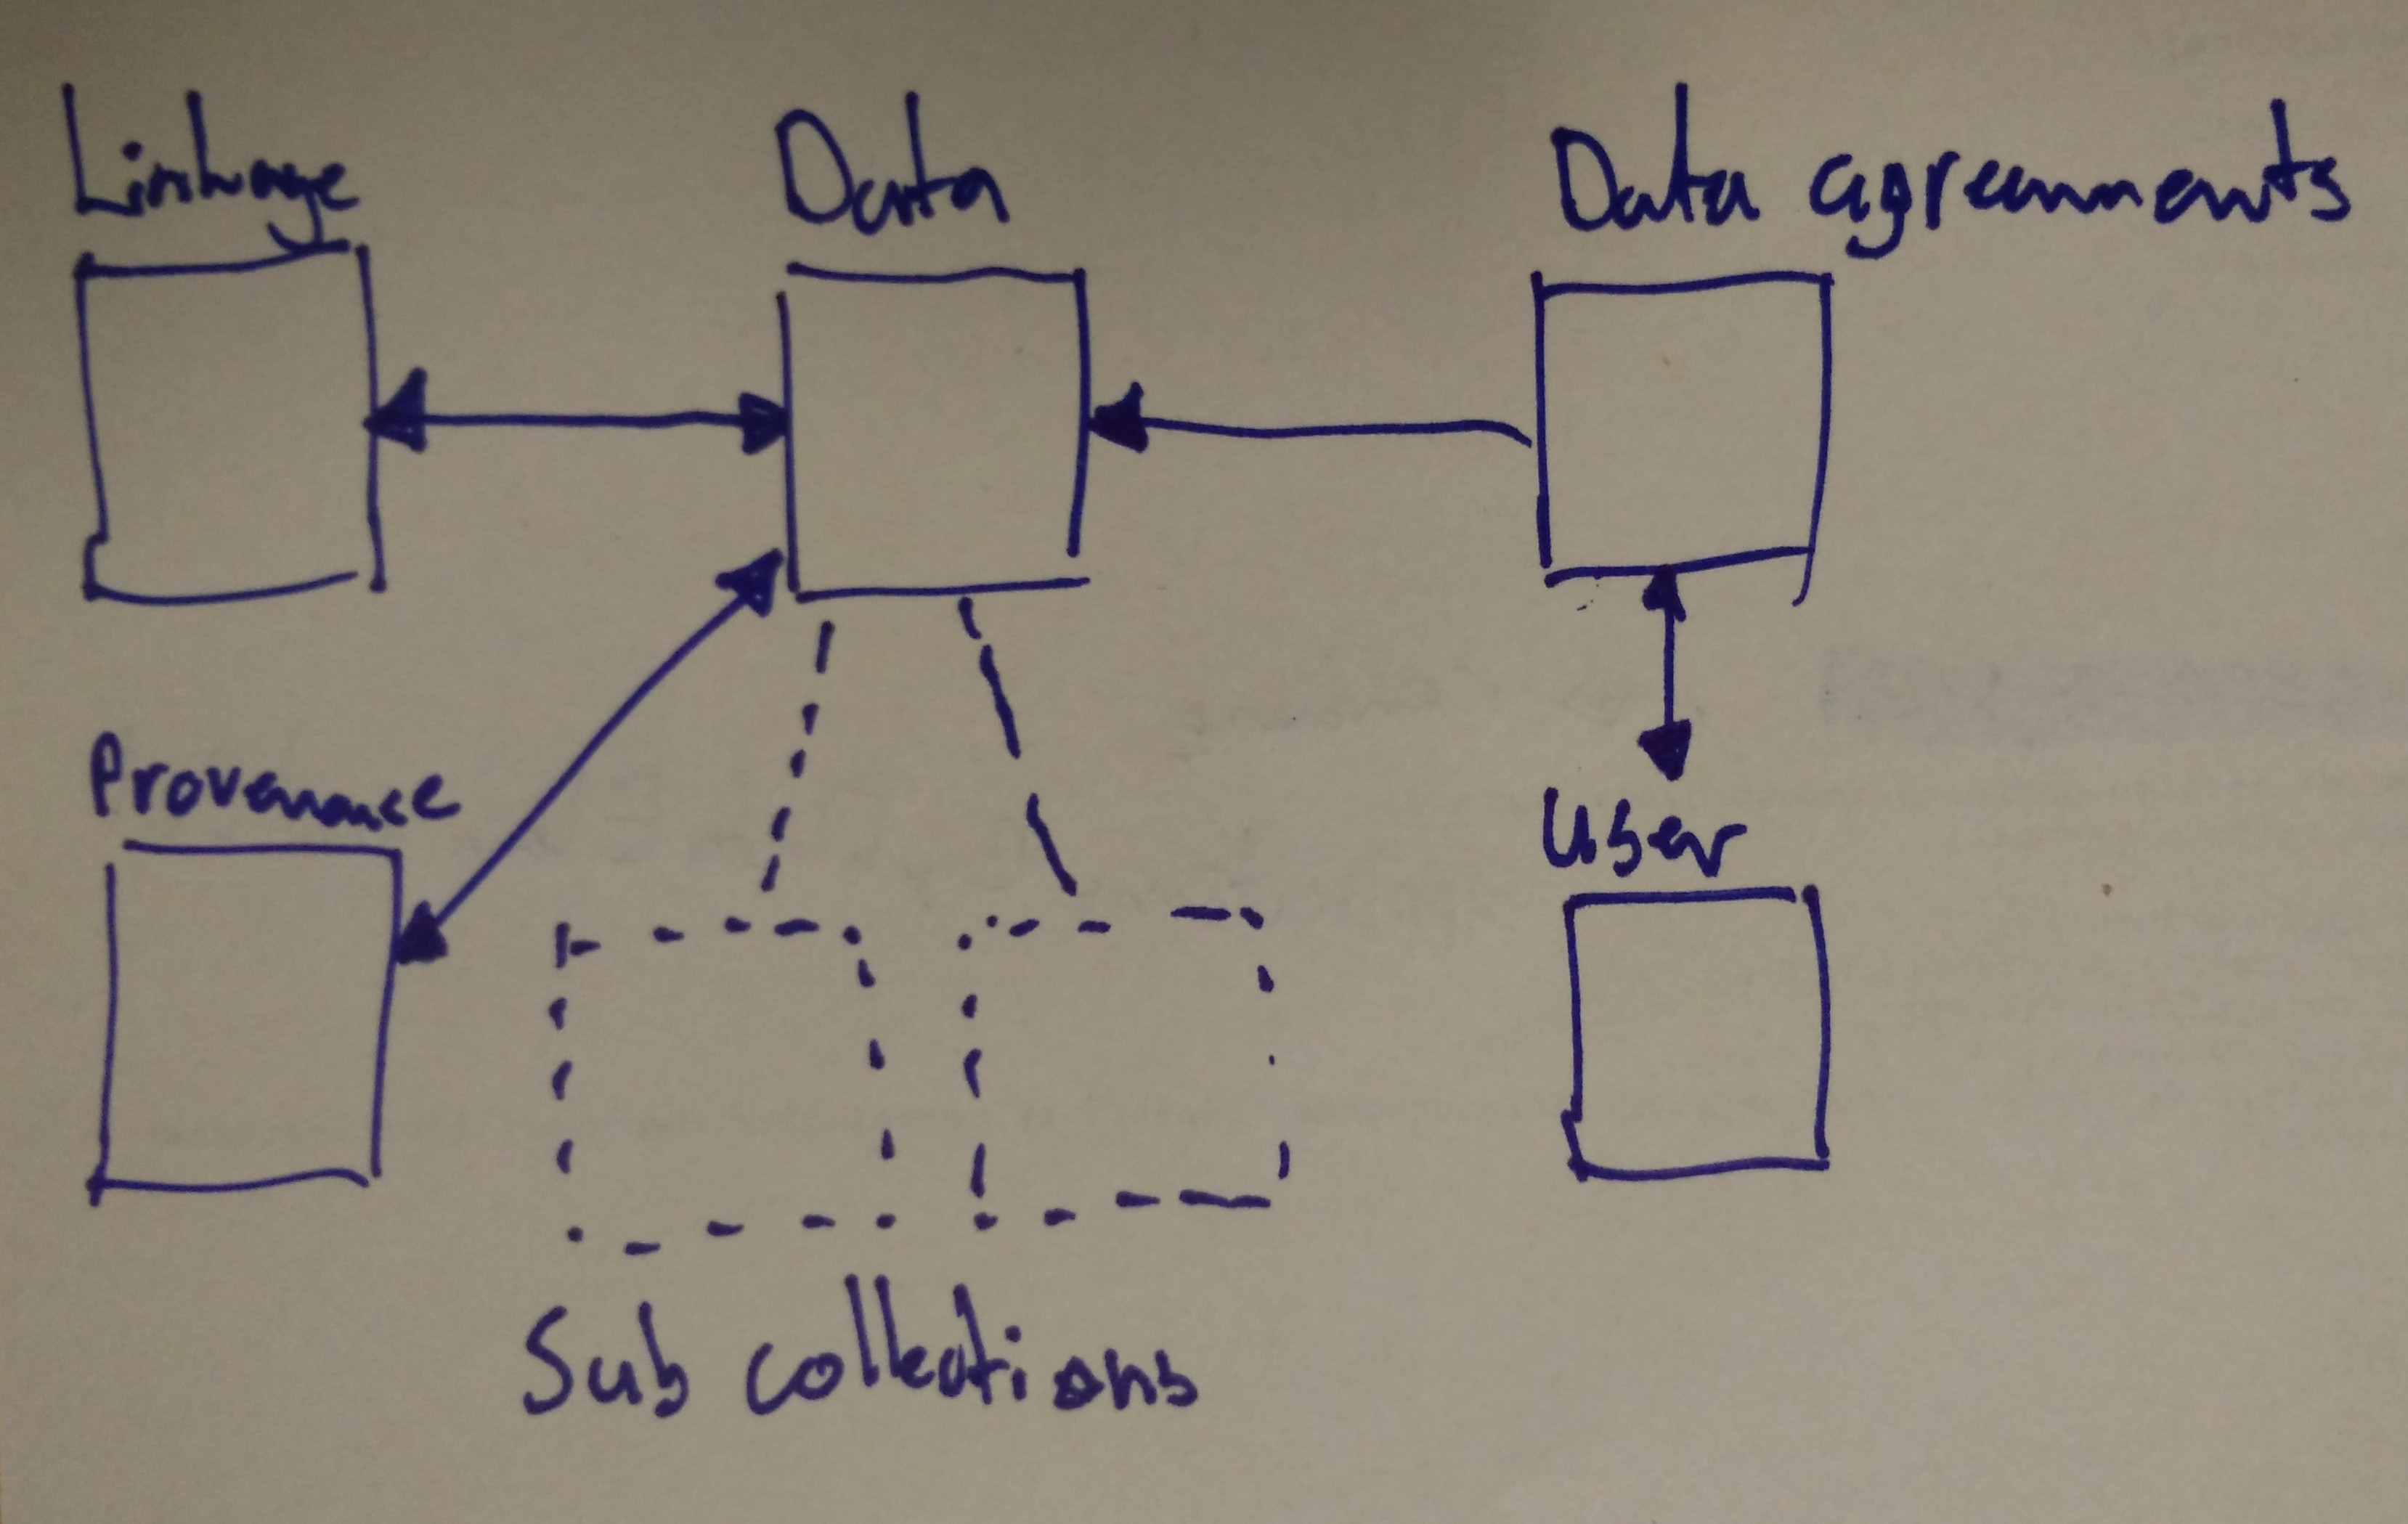
\includegraphics[width=1.0\linewidth]{images/small-structure-v2}
	\caption{Initial drawing of the data model} %TODO: write more caption
	\label{fig:model-drawing}
\end{figure}

\paragraph{Schema(less)}
\label{datamodel-schema}

A choice which is made later in the software engineering part of the project is whether or not to pick a schemaless database.
This point will be elaborated further on in this thesis.
For now it will suffice to say that the identified requirement 3 asks for a schemaless database.

%Part of introduction?
\section{Data Gathering}
\label{datamodel-gathering}

%TODO: compile list of problems

%TODO: what is provenance (literature) and how do I model this?